
\section{Evaluasi}
\subsection{Lingkungan Pengujian}
4 digitalocean cpu based, 1 openssl basic 1 core, 1core, 16core, 32core. Semua pake OS, apache versi yang sama
\begin{figure}[h]
  \centering
  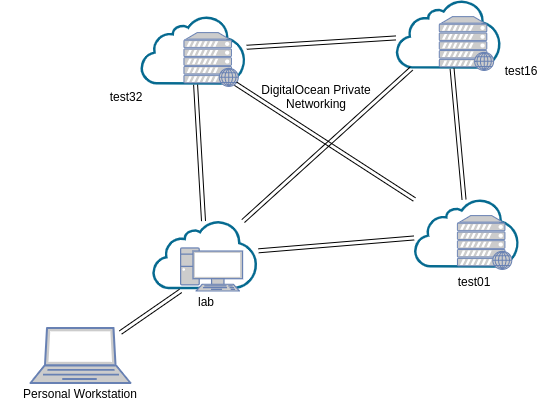
\includegraphics[width=0.8\textwidth]{resources/ch-4/testing_arch.png}
  \caption{Arsitektur Lingkungan Pengujian}
  \label{fig:testing_arch}
\end{figure}

\subsection{Skenario Pengujian}
Install apache, test pake apachebench, get waktu, rata2 tiga kali
\subsection{Hasil dan Analisis}
\subsubsection{Hasil Pengujian}
  Langsung data speedup aja, data raw simpen di lampiran

  \begin{table}[ht]
  \caption{Test table} % title of Table
  \centering % used for centering table
  \begin{tabular}{c c c c} % centered columns (4 columns)
  \hline\hline %inserts double horizontal lines
  Case & Method\#1 & Method\#2 & Method\#3 \\ [0.5ex] % inserts table
  %heading
  \hline % inserts single horizontal line
  1 & 50 & 837 & 970 \\ % inserting body of the table
  2 & 47 & 877 & 230 \\
  3 & 31 & 25 & 415 \\
  4 & 35 & 144 & 2356 \\
  5 & 45 & 300 & 556 \\ [1ex] % [1ex] adds vertical space
  \hline %inserts single line
  \end{tabular}
  \label{table:nonlin} % is used to refer this table in the text
  \end{table}

\subsubsection{Analisis Pengujian}
